%% bare_conf.tex
%% V1.4b
%% 2015/08/26
%% by Michael Shell
%% See:
%% http://www.michaelshell.org/
%% for current contact information.
%%
%% This is a skeleton file demonstrating the use of IEEEtran.cls
%% (requires IEEEtran.cls version 1.8b or later) with an IEEE
%% conference paper.
%%
%% Support sites:
%% http://www.michaelshell.org/tex/ieeetran/
%% http://www.ctan.org/pkg/ieeetran
%% and
%% http://www.ieee.org/

%%*************************************************************************
%% Legal Notice:
%% This code is offered as-is without any warranty either expressed or
%% implied; without even the implied warranty of MERCHANTABILITY or
%% FITNESS FOR A PARTICULAR PURPOSE! 
%% User assumes all risk.
%% In no event shall the IEEE or any contributor to this code be liable for
%% any damages or losses, including, but not limited to, incidental,
%% consequential, or any other damages, resulting from the use or misuse
%% of any information contained here.
%%
%% All comments are the opinions of their respective authors and are not
%% necessarily endorsed by the IEEE.
%%
%% This work is distributed under the LaTeX Project Public License (LPPL)
%% ( http://www.latex-project.org/ ) version 1.3, and may be freely used,
%% distributed and modified. A copy of the LPPL, version 1.3, is included
%% in the base LaTeX documentation of all distributions of LaTeX released
%% 2003/12/01 or later.
%% Retain all contribution notices and credits.
%% ** Modified files should be clearly indicated as such, including  **
%% ** renaming them and changing author support contact information. **
%%*************************************************************************


% *** Authors should verify (and, if needed, correct) their LaTeX system  ***
% *** with the testflow diagnostic prior to trusting their LaTeX platform ***
% *** with production work. The IEEE's font choices and paper sizes can   ***
% *** trigger bugs that do not appear when using other class files.       ***                          ***
% The testflow support page is at:
% http://www.michaelshell.org/tex/testflow/



% Format guidelines for ECE695/CS590 final report
\documentclass[11pt, draftclsnofoot, onecolumn]{IEEEtran}

% \documentclass[conference]{IEEEtran}
% Some Computer Society conferences also require the compsoc mode option,
% but others use the standard conference format.
%
% If IEEEtran.cls has not been installed into the LaTeX system files,
% manually specify the path to it like:
% \documentclass[conference]{../sty/IEEEtran}

% ebarsallo
% Custom (check the validity of this customization if decided to submit this as a paper.
% Just to be able to color hint text.
\usepackage{color}

% listings
\usepackage{listings}
\lstset{
	language=Java,
	aboveskip=3mm,
	belowskip=3mm,
	showstringspaces=false,
	columns=flexible,
	basicstyle={\small\ttfamily},
	numberstyle=\small,
	breaklines=true,
	breakatwhitespace=true,
	tabsize=3
}

% tabbles
\usepackage{multirow}

% Table label (not ALL CAPS)
\def\tablename{Table}

% SI units
\usepackage{siunitx}

% Some very useful LaTeX packages include:
% (uncomment the ones you want to load)


% *** MISC UTILITY PACKAGES ***
%
%\usepackage{ifpdf}
% Heiko Oberdiek's ifpdf.sty is very useful if you need conditional
% compilation based on whether the output is pdf or dvi.
% usage:
% \ifpdf
%   % pdf code
% \else
%   % dvi code
% \fi
% The latest version of ifpdf.sty can be obtained from:
% http://www.ctan.org/pkg/ifpdf
% Also, note that IEEEtran.cls V1.7 and later provides a builtin
% \ifCLASSINFOpdf conditional that works the same way.
% When switching from latex to pdflatex and vice-versa, the compiler may
% have to be run twice to clear warning/error messages.






% *** CITATION PACKAGES ***
%
%\usepackage{cite}
% cite.sty was written by Donald Arseneau
% V1.6 and later of IEEEtran pre-defines the format of the cite.sty package
% \cite{} output to follow that of the IEEE. Loading the cite package will
% result in citation numbers being automatically sorted and properly
% "compressed/ranged". e.g., [1], [9], [2], [7], [5], [6] without using
% cite.sty will become [1], [2], [5]--[7], [9] using cite.sty. cite.sty's
% \cite will automatically add leading space, if needed. Use cite.sty's
% noadjust option (cite.sty V3.8 and later) if you want to turn this off
% such as if a citation ever needs to be enclosed in parenthesis.
% cite.sty is already installed on most LaTeX systems. Be sure and use
% version 5.0 (2009-03-20) and later if using hyperref.sty.
% The latest version can be obtained at:
% http://www.ctan.org/pkg/cite
% The documentation is contained in the cite.sty file itself.






% *** GRAPHICS RELATED PACKAGES ***
%
\ifCLASSINFOpdf
 \usepackage[pdftex]{graphicx}
% declare the path(s) where your graphic files are
 \graphicspath{{imgs/}}
% and their extensions so you won't have to specify these with
% every instance of \includegraphics
 \DeclareGraphicsExtensions{.pdf,.jpeg,.png}
\else
% or other class option (dvipsone, dvipdf, if not using dvips). graphicx
% will default to the driver specified in the system graphics.cfg if no
% driver is specified.
% \usepackage[dvips]{graphicx}
% declare the path(s) where your graphic files are
% \graphicspath{{../eps/}}
% and their extensions so you won't have to specify these with
% every instance of \includegraphics
% \DeclareGraphicsExtensions{.eps}
\fi
% graphicx was written by David Carlisle and Sebastian Rahtz. It is
% required if you want graphics, photos, etc. graphicx.sty is already
% installed on most LaTeX systems. The latest version and documentation
% can be obtained at: 
% http://www.ctan.org/pkg/graphicx
% Another good source of documentation is "Using Imported Graphics in
% LaTeX2e" by Keith Reckdahl which can be found at:
% http://www.ctan.org/pkg/epslatex
%
% latex, and pdflatex in dvi mode, support graphics in encapsulated
% postscript (.eps) format. pdflatex in pdf mode supports graphics
% in .pdf, .jpeg, .png and .mps (metapost) formats. Users should ensure
% that all non-photo figures use a vector format (.eps, .pdf, .mps) and
% not a bitmapped formats (.jpeg, .png). The IEEE frowns on bitmapped formats
% which can result in "jaggedy"/blurry rendering of lines and letters as
% well as large increases in file sizes.
%
% You can find documentation about the pdfTeX application at:
% http://www.tug.org/applications/pdftex





% *** MATH PACKAGES ***
%
%\usepackage{amsmath}
% A popular package from the American Mathematical Society that provides
% many useful and powerful commands for dealing with mathematics.
%
% Note that the amsmath package sets \interdisplaylinepenalty to 10000
% thus preventing page breaks from occurring within multiline equations. Use:
%\interdisplaylinepenalty=2500
% after loading amsmath to restore such page breaks as IEEEtran.cls normally
% does. amsmath.sty is already installed on most LaTeX systems. The latest
% version and documentation can be obtained at:
% http://www.ctan.org/pkg/amsmath





% *** SPECIALIZED LIST PACKAGES ***
%
%\usepackage{algorithmic}
% algorithmic.sty was written by Peter Williams and Rogerio Brito.
% This package provides an algorithmic environment fo describing algorithms.
% You can use the algorithmic environment in-text or within a figure
% environment to provide for a floating algorithm. Do NOT use the algorithm
% floating environment provided by algorithm.sty (by the same authors) or
% algorithm2e.sty (by Christophe Fiorio) as the IEEE does not use dedicated
% algorithm float types and packages that provide these will not provide
% correct IEEE style captions. The latest version and documentation of
% algorithmic.sty can be obtained at:
% http://www.ctan.org/pkg/algorithms
% Also of interest may be the (relatively newer and more customizable)
% algorithmicx.sty package by Szasz Janos:
% http://www.ctan.org/pkg/algorithmicx




% *** ALIGNMENT PACKAGES ***
%
%\usepackage{array}
% Frank Mittelbach's and David Carlisle's array.sty patches and improves
% the standard LaTeX2e array and tabular environments to provide better
% appearance and additional user controls. As the default LaTeX2e table
% generation code is lacking to the point of almost being broken with
% respect to the quality of the end results, all users are strongly
% advised to use an enhanced (at the very least that provided by array.sty)
% set of table tools. array.sty is already installed on most systems. The
% latest version and documentation can be obtained at:
% http://www.ctan.org/pkg/array


% IEEEtran contains the IEEEeqnarray family of commands that can be used to
% generate multiline equations as well as matrices, tables, etc., of high
% quality.




% *** SUBFIGURE PACKAGES ***
%\ifCLASSOPTIONcompsoc
%  \usepackage[caption=false,font=normalsize,labelfont=sf,textfont=sf]{subfig}
%\else
%  \usepackage[caption=false,font=footnotesize]{subfig}
%\fi
% subfig.sty, written by Steven Douglas Cochran, is the modern replacement
% for subfigure.sty, the latter of which is no longer maintained and is
% incompatible with some LaTeX packages including fixltx2e. However,
% subfig.sty requires and automatically loads Axel Sommerfeldt's caption.sty
% which will override IEEEtran.cls' handling of captions and this will result
% in non-IEEE style figure/table captions. To prevent this problem, be sure
% and invoke subfig.sty's "caption=false" package option (available since
% subfig.sty version 1.3, 2005/06/28) as this is will preserve IEEEtran.cls
% handling of captions.
% Note that the Computer Society format requires a larger sans serif font
% than the serif footnote size font used in traditional IEEE formatting
% and thus the need to invoke different subfig.sty package options depending
% on whether compsoc mode has been enabled.
%
% The latest version and documentation of subfig.sty can be obtained at:
% http://www.ctan.org/pkg/subfig




% *** FLOAT PACKAGES ***
%
%\usepackage{fixltx2e}
% fixltx2e, the successor to the earlier fix2col.sty, was written by
% Frank Mittelbach and David Carlisle. This package corrects a few problems
% in the LaTeX2e kernel, the most notable of which is that in current
% LaTeX2e releases, the ordering of single and double column floats is not
% guaranteed to be preserved. Thus, an unpatched LaTeX2e can allow a
% single column figure to be placed prior to an earlier double column
% figure.
% Be aware that LaTeX2e kernels dated 2015 and later have fixltx2e.sty's
% corrections already built into the system in which case a warning will
% be issued if an attempt is made to load fixltx2e.sty as it is no longer
% needed.
% The latest version and documentation can be found at:
% http://www.ctan.org/pkg/fixltx2e


%\usepackage{stfloats}
% stfloats.sty was written by Sigitas Tolusis. This package gives LaTeX2e
% the ability to do double column floats at the bottom of the page as well
% as the top. (e.g., "\begin{figure*}[!b]" is not normally possible in
% LaTeX2e). It also provides a command:
%\fnbelowfloat
% to enable the placement of footnotes below bottom floats (the standard
% LaTeX2e kernel puts them above bottom floats). This is an invasive package
% which rewrites many portions of the LaTeX2e float routines. It may not work
% with other packages that modify the LaTeX2e float routines. The latest
% version and documentation can be obtained at:
% http://www.ctan.org/pkg/stfloats
% Do not use the stfloats baselinefloat ability as the IEEE does not allow
% \baselineskip to stretch. Authors submitting work to the IEEE should note
% that the IEEE rarely uses double column equations and that authors should try
% to avoid such use. Do not be tempted to use the cuted.sty or midfloat.sty
% packages (also by Sigitas Tolusis) as the IEEE does not format its papers in
% such ways.
% Do not attempt to use stfloats with fixltx2e as they are incompatible.
% Instead, use Morten Hogholm'a dblfloatfix which combines the features
% of both fixltx2e and stfloats:
%
% \usepackage{dblfloatfix}
% The latest version can be found at:
% http://www.ctan.org/pkg/dblfloatfix




% *** PDF, URL AND HYPERLINK PACKAGES ***
%
\usepackage{url}
% url.sty was written by Donald Arseneau. It provides better support for
% handling and breaking URLs. url.sty is already installed on most LaTeX
% systems. The latest version and documentation can be obtained at:
% http://www.ctan.org/pkg/url
% Basically, \url{my_url_here}.




% *** Do not adjust lengths that control margins, column widths, etc. ***
% *** Do not use packages that alter fonts (such as pslatex).         ***
% There should be no need to do such things with IEEEtran.cls V1.6 and later.
% (Unless specifically asked to do so by the journal or conference you plan
% to submit to, of course. )


% correct bad hyphenation here
\hyphenation{op-tical net-works semi-conduc-tor}

\usepackage{multicol}

\begin{document}
	%
	% paper title
	% Titles are generally capitalized except for words such as a, an, and, as,
	% at, but, by, for, in, nor, of, on, or, the, to and up, which are usually
	% not capitalized unless they are the first or last word of the title.
	% Linebreaks \\ can be used within to get better formatting as desired.
	% Do not put math or special symbols in the title.
	\title{How to Make Today's Weareable Health Devices more Trustable}
	
	
	% author names and affiliations
	% use a multiple column layout for up to three different
	% affiliations
	%\author{\IEEEauthorblockN{Michael Shell}
	%	\IEEEauthorblockA{School of Electrical and\\Computer Engineering\\
	%		Georgia Institute of Technology\\
	%		Atlanta, Georgia 30332--0250\\
	%		Email: http://www.michaelshell.org/contact.html}
	%	\and
	%	\IEEEauthorblockN{Homer Simpson}
	%	\IEEEauthorblockA{Twentieth Century Fox\\
	%		Springfield, USA\\
	%		Email: homer@thesimpsons.com}
	%	\and
	%	\IEEEauthorblockN{James Kirk\\ and Montgomery Scott}
	%	\IEEEauthorblockA{Starfleet Academy\\
	%		San Francisco, California 96678--2391\\
	%		Telephone: (800) 555--1212\\
	%		Fax: (888) 555--1212}}
	
	\author{Naixing Wang, Edgardo Barsallo}
	
	% conference papers do not typically use \thanks and this command
	% is locked out in conference mode. If really needed, such as for
	% the acknowledgment of grants, issue a \IEEEoverridecommandlockouts
	% after \documentclass
	
	% for over three affiliations, or if they all won't fit within the width
	% of the page, use this alternative format:
	% 
	%\author{\IEEEauthorblockN{Michael Shell\IEEEauthorrefmark{1},
	%Homer Simpson\IEEEauthorrefmark{2},
	%James Kirk\IEEEauthorrefmark{3}, 
	%Montgomery Scott\IEEEauthorrefmark{3} and
	%Eldon Tyrell\IEEEauthorrefmark{4}}
	%\IEEEauthorblockA{\IEEEauthorrefmark{1}School of Electrical and Computer Engineering\\
	%Georgia Institute of Technology,
	%Atlanta, Georgia 30332--0250\\ Email: see http://www.michaelshell.org/contact.html}
	%\IEEEauthorblockA{\IEEEauthorrefmark{2}Twentieth Century Fox, Springfield, USA\\
	%Email: homer@thesimpsons.com}
	%\IEEEauthorblockA{\IEEEauthorrefmark{3}Starfleet Academy, San Francisco, California 96678-2391\\
	%Telephone: (800) 555--1212, Fax: (888) 555--1212}
	%\IEEEauthorblockA{\IEEEauthorrefmark{4}Tyrell Inc., 123 Replicant Street, Los Angeles, California 90210--4321}}
	
	
	% use for special paper notices
	%\IEEEspecialpapernotice{(Invited Paper)}
	
	
	
	
	% make the title area
	\maketitle
	
	% As a general rule, do not put math, special symbols or citations
	% in the abstract
	%\begin{abstract}
	%	The abstract goes here.
	%\end{abstract}
	
	% no keywords
	
	
	
	
	% For peer review papers, you can put extra information on the cover
	% page as needed:
	% \ifCLASSOPTIONpeerreview
	% \begin{center} \bfseries EDICS Category: 3-BBND \end{center}
	% \fi
	%
	% For peerreview papers, this IEEEtran command inserts a page break and
	% creates the second title. It will be ignored for other modes.
	\IEEEpeerreviewmaketitle
	
	\section{Introduction} \label{sec:Introduction} % [2-3 pages]
	% no \IEEEPARstart
	%This demo file is intended to serve as a ``starter file''
	%for IEEE conference papers produced under \LaTeX\ using
	%IEEEtran.cls version 1.8b and later.
	% You must have at least 2 lines in the paragraph with the drop letter
	% (should never be an issue)
	%I wish you the best of success.
	
	%\hfill mds
	%\hfill August 26, 2015
	
	% 1.1 What is the problem?
    Wearable devices has increased in popularity as people are starting to use more frequently for their fitness. Typical uses include calories tracker, workout assistant or step counters. Even tough these wearable devices can measure many other healthy signals (e.g. heart rate), they are still not perceived as reliable. Specifically, the accuracy for measure the heart rate varies from device to device. This project is aimed to analyze this from the hardware and software perspective.
    
    Wearable devices monitor heart rate by recording the photoplethysmography (PPG) signal from the skin. A PPG signal is obtained by illuminating skin using a light-emitting diode and detecting the intensity changes in the reflected light. Hence the periodicity of the PPG signal represents the heart rate. However, PPG signals are highly contaminated by artifacts caused by movements of the subject. Such motion artifacts strongly interfere with heart rate especially in fitness applications when the PPG signal is recorded during physical exercise of the subject. The situation gets worse in the case considered in this letter when the PPG signals are recorded from wrist. Such PPG signals experience severe motion artifacts due to the loose interface between the PPG sensor and skin.
    
    % 1.2 How has it been solved till now?
    Many related work proposed so far for motion artifacts analysis and reduction consider weak motion artifacts scenarios in~\cite{couceiro2014detection, kim2007adaptive, santos2012accelerometer, lee2013comparison}. In~\cite{couceiro2014detection}, multiple algorithms for improving the accuracy of heart rate monitoring are presented. In~\cite{kim2007adaptive}, the relation between the PPG signal and the accelerometer data is analyzed. In~\cite{santos2012accelerometer}, a method for long-term monitoring of vital signs tested during physical exercise is developed. The results show that the system has potential to monitor cardiac activity at moderate speed (up to 4 km/h), but with increasing speed (i.e. running) the motion artifacts dominate the PPG. In~\cite{lee2013comparison}, the accuracy of heart rate monitoring with PPG signal using different wavelength of lights (red, green and blue) is analyzed. The results show that the green light PPG has a higher accuracy and a much larger signal noise ratio. 
    
    % 1.3 What was your main solution idea?
    % 1.4 What are the key technical details of your solution? 
    Although heart rate monitoring from wrist-type PPG signals during intensive physical exercise is extremely challenging, but it is of great interest to wearable smart devices such as smartwatches. In this paper, we analyze the reliability of Motorola Moto 360 (2nd Gen.). We also compare the accuracy of heart rate monitoring between Moto 360 (2nd Gen.) and Apple Watch, which is the dominated smartwatch in the market~\cite{IDC2016WearableQ3}. We use a  medical fingertip pulse oximeter as base reference to analyze the accuracy of the  two  devices. To further study the relation between PPG signal and accelerometer data, we compare the PPG signal with acceleration on each axis using correlation coefficient.
    
    In addition, we analyze the reliability of Android Wear 1.0 by using a black box testing approach. Fuzz testing is a cost effective technique that can allow to test a great range program in a relative short time. Besides, by fuzz the input (either by randomly generate data or by mutate data from a previous valid input) we can stress applications and identify most of common bugs. 
    
    % 1.5 How did you evaluate your solution (2-3 key results)? 
    % 1.6 A high level figure of your solution, or evaluation method 
    % Not sure we have address this so far.
    
    % 1.7 A list of contributions (3-4) that you can claim from this work. 
    This work represent some of the few initiatives that address the reliability of Android wearable devices, and its contributions are outlined below:
    
    \begin{enumerate}
    \item \textbf{A correlation study between the PPG signal and body motion}. Our experiments concluded that there is an important correlation between the PPG signal and x-axis acceleration. This results could be used to improve the wearable reliability.
    \item \textbf{A guideline to improve the accuracy of the heart rate monitor on Android Wear}. By following the concluded recommendations of our work, the accuracy of the Motorola Moto 360 (2nd Gen.) can be improved. 
    \item \textbf{The study on the reliability of the Android Wear 1.0}. An important study of the reliability of the built-in apps included on the Motorola Moto 360 (2nd Gen.) is introduced, which could aid to improve the perceived reliability from the wearable.
    \end{enumerate}
    
    This paper is organized as follows. Section II reviews concepts that are relevant to this paper. Section III-V describes the details of solution from hardware and software perspective. Conclusions and future work are described in Section VI and Section VII respectively.
    
	%\subsection{Subsection Heading Here}
	%Subsection text here.
	
	%\subsubsection{Subsubsection Heading Here}
	%Subsubsection text here.
	
	
	% An example of a floating figure using the graphicx package.
	% Note that \label must occur AFTER (or within) \caption.
	% For figures, \caption should occur after the \includegraphics.
	% Note that IEEEtran v1.7 and later has special internal code that
	% is designed to preserve the operation of \label within \caption
	% even when the captionsoff option is in effect. However, because
	% of issues like this, it may be the safest practice to put all your
	% \label just after \caption rather than within \caption{}.
	%
	% Reminder: the "draftcls" or "draftclsnofoot", not "draft", class
	% option should be used if it is desired that the figures are to be
	% displayed while in draft mode.
	%
	%\begin{figure}[!t]
	%\centering
	%\includegraphics[width=2.5in]{myfigure}
	% where an .eps filename suffix will be assumed under latex, 
	% and a .pdf suffix will be assumed for pdflatex; or what has been declared
	% via \DeclareGraphicsExtensions.
	%\caption{Simulation results for the network.}
	%\label{fig_sim}
	%\end{figure}
	
	% Note that the IEEE typically puts floats only at the top, even when this
	% results in a large percentage of a column being occupied by floats.
	
	
	% An example of a double column floating figure using two subfigures.
	% (The subfig.sty package must be loaded for this to work.)
	% The subfigure \label commands are set within each subfloat command,
	% and the \label for the overall figure must come after \caption.
	% \hfil is used as a separator to get equal spacing.
	% Watch out that the combined width of all the subfigures on a 
	% line do not exceed the text width or a line break will occur.
	%
	%\begin{figure*}[!t]
	%\centering
	%\subfloat[Case I]{\includegraphics[width=2.5in]{box}%
	%\label{fig_first_case}}
	%\hfil
	%\subfloat[Case II]{\includegraphics[width=2.5in]{box}%
	%\label{fig_second_case}}
	%\caption{Simulation results for the network.}
	%\label{fig_sim}
	%\end{figure*}
	%
	% Note that often IEEE papers with subfigures do not employ subfigure
	% captions (using the optional argument to \subfloat[]), but instead will
	% reference/describe all of them (a), (b), etc., within the main caption.
	% Be aware that for subfig.sty to generate the (a), (b), etc., subfigure
	% labels, the optional argument to \subfloat must be present. If a
	% subcaption is not desired, just leave its contents blank,
	% e.g., \subfloat[].
	
	
	% An example of a floating table. Note that, for IEEE style tables, the
	% \caption command should come BEFORE the table and, given that table
	% captions serve much like titles, are usually capitalized except for words
	% such as a, an, and, as, at, but, by, for, in, nor, of, on, or, the, to
	% and up, which are usually not capitalized unless they are the first or
	% last word of the caption. Table text will default to \footnotesize as
	% the IEEE normally uses this smaller font for tables.
	% The \label must come after \caption as always.
	%
	%\begin{table}[!t]
	%% increase table row spacing, adjust to taste
	%\renewcommand{\arraystretch}{1.3}
	% if using array.sty, it might be a good idea to tweak the value of
	% \extrarowheight as needed to properly center the text within the cells
	%\caption{An Example of a Table}
	%\label{table_example}
	%\centering
	%% Some packages, such as MDW tools, offer better commands for making tables
	%% than the plain LaTeX2e tabular which is used here.
	%\begin{tabular}{|c||c|}
	%\hline
	%One & Two\\
	%\hline
	%Three & Four\\
	%\hline
	%\end{tabular}
	%\end{table}
	
	
	% Note that the IEEE does not put floats in the very first column
	% - or typically anywhere on the first page for that matter. Also,
	% in-text middle ("here") positioning is typically not used, but it
	% is allowed and encouraged for Computer Society conferences (but
	% not Computer Society journals). Most IEEE journals/conferences use
	% top floats exclusively. 
	% Note that, LaTeX2e, unlike IEEE journals/conferences, places
	% footnotes above bottom floats. This can be corrected via the
	% \fnbelowfloat command of the stfloats package.
	
    \pagebreak
	\section{Background} \label{sec:Background} %[2-3 pages]
	% 2.1 Provide a background of the problem, in easy-to-understand terms. This should not be tied to your solution. Here you can provide some context about the problem – why it is important, where it is used, etc.
	Wearable devices embedded with heart rate sensors, which are based on photoplethysmography (PPG), have become increasingly popular. More than ten companies produce these wearable devices commercially. The principle of PPG has been reviewed previously~\cite{tamura2014wearable}, and is explained briefly here. Light traveling though biological tissue can be absorbed by different substances, including pigments in the skin, bone, and arterial and venous blood. Most changes in blood flow occur mainly in the arteries and arterioles (but not in the veins). For example, arteries contain more blood volume during the systolic phase of the cardiac cycle than during the diastolic phase. PPG sensors optically detect changes in the blood flow volume (i.e., changes in the detected light intensity) in the micro-vascular bed of tissue via reflection from or transmission through the tissue. The changes in light intensity are associated with small variations in blood perfusion of the tissue and provide information on the cardiovascular system, in particular, the heart rate. Due to the simplicity of this device, wearable PPG heart rate sensors have been developed.
    
    The sensor system consists of a light source and a detector, with green, red and infrared (IR) light-emitting diodes (LEDs) commonly used as the light source. Blood absorbs more light than the surrounding tissue. Therefore, a reduction in the amount of blood is detected as an increase in the intensity of the detected light. The wavelength and distance between the light source and photo diode (PD) determine the penetration depth of the light. Green light is suitable for the measurement of superficial blood flow in skin. IR or near-IR wavelengths are better for measurement of deep-tissue blood flow (e.g., blood flow in muscles). However, a green LED has much greater absorptivity for both oxyhaemoglobin and deoxyhaemoglobin compared to infrared light. Therefore, the change in reflected green light is greater than that in reflected infrared light when blood pulses through the skin, resulting in a better signal-to-noise ratio for the green light source. Therefore, green-wavelength PPG devices are becoming increasingly popular due to the large intensity variations in modulation observed during the cardiac cycle for these wavelengths~\cite{lee2013comparison}.
    
    Typically, the wearable PPG has two modes, which are transmission and reflectance. In transmission mode, the light transmitted through the medium is detected by a PD opposite the LED source, while in reflectance mode, the PD detects light that is back-scattered or reflected from tissue, bone and/or blood vessels.The transmission mode is capable of obtaining a relatively good signal, but the measurement site may be limited. Reflectance mode eliminates the problems associated with sensor placement. Therefore, the use of reflectance mode is typical for wearable devices. However, reflection-mode PPG is affected by motion artifacts. Any movement, such as physical activity, may lead to motion artifacts that corrupt the PPG signal and limit the measurement accuracy of physiological parameters [Reference].
    
    In this project, we analyze the reliability of Motorola Moto 360 (2nd Gen.), which heart rate monitors follows a reflection-mode PPG. Furthermore, the PPG sensor embedded in the smartwatch is NJL5513R, which provides one red LED, one infrared LED and two green LEDs to be used for heart rate~\cite{NJL5513Rdatasheet}. Nevertheless, experiments demonstrate that Motorola Moto 306 (2nd Gen.) uses two green LEDs to monitor the users heart rate.
    
    % 2.2 Give a high level view of the different approaches used to solve the problem till now. Within each approach, there may be multiple papers that fall within the same approach.
    
    Various attempts have been made to find strategies to circumvent the motion artifacts~\cite{couceiro2014detection}. In ~\cite{kim2007adaptive}, the relation between the PPG signal and the accelerometer data is analyzed. A PPG sensor with accelerometer is placed on the forehead. The subject is then asked to shake his head in each of the axes of the accelerometer, thereby finding the corresponding correlation for all axes. In ~\cite{santos2012accelerometer}, a method for long-term monitoring of vital signs tested during physical exercise is developed. The results show that the system has potential to monitor cardiac activity at moderate speed (up to 4 km/h), but with increasing speed (i.e. running) the motion artifacts dominate the PPG. In ~\cite{lee2013comparison}, the accuracy of heart rate monitoring with PPG signal using different wavelength of lights (red, green and blue) is analyzed. The results show that the green light PPG has a higher accuracy and a much larger signal noise ratio. Therefore, the green light could be a more suitable method than red and blue light PPG for monitoring HR in normal daily life.
    
    A different strategy is used by Apple. In Apple watch, it attempts to measure your heart rate every 10 minutes, but will not record it when the person is in motion or his/her arm is moving~\cite{AppleHeartRate2015}. This mechanism can improve the overall accuracy of the data it collected.

	\section{Solution} \label{sec:Solution}
	% Here you describe the detailed techniques in your solution. For each part of the solution, put it in the context of the overall system or solution – where does it fit, what is its functionality. Do not just give pseudo code, but explain in words what is the design behind the technique. If there are alternate ways of doing this, describe them and say why one is better than the others. If your technique expands some prior technique, refer to that, and point out the addition that you have done. 

%citation needed: Motorola Moto 360 (2nd Gen) considered one of the best.
As described in the \S 1, to analyze the reliability of wearable devices, the study is done from two different perspectives: hardware and software. On both perspectives, the target of the analysis and experiments is the Motorola Moto 360 (2nd Gen.), released on 2015 and considered one of the best android wear smart watch~\cite{BestAW2016}. Then, from the hardware perspective, the study is focused on the heart rate monitor. We analyzed the accuracy of the measures obtained from the heart rate sensor, TI AFE4404 ~\cite{AFE4404dev}, and study the factors that affects its precision. By the other hand, from the software perspective, we validate the reliability of the Android wearable by applying black box testing using fuzz techniques.

The following sections describe in detail the design and implementation overtaken, and the different experiments with their respective results done from each of the perspective. 

	\section{Hardware} \label{sec:Hardware}
    
    \subsection{Related Work} \label{subsec:HardwareRelatedWork}
    % Existing solutions
    In this section, we describe the related work for the analysis of the reliability of the Motorola Moto 360 (2nd Gen.). Apple Watch series 1 is a commercial smartwatch that was released in April, 2015, and dominates the wearable market~\cite{IDC2016WearableQ3}. Apple Watch also provides the feature of heart rate monitoring, and according previous studies has shown that this smartwatch has accuracy compare with other more specialized devices (e.g. Fitbit Charge HR, Polar H7 chest strap)~\cite{TomGuideHRComparison2015}. In our experiments, we compare the accuracy of heart rate monitoring between Motorola Moto 360 (2nd Gen.) and Apple watch. We also use a medical fingertip pulse oximeter (Santamedical Generation 2 SM-165) as base reference to analyze the accuracy of the two wearable devices. Santamedical SM-165 is a fingertip pulse oximeter with oximetry blood oxygen saturation monitoring feature. The precision of Santamedical g2 SM-165 is $\pm2$ BPM (Beats per Minutes)~\cite{SantamedicalSM165}. To further study the accuracy of the Motorola Moto 360 (2nd Gen.), we compared the relation between the PPG signal and the accelerometer signal on each axis. Details are described in next subsection.
    
	\subsection{Design and Implementation} \label{subsec:HarwareDesignImpl} % [1-3 pages]
	% Design
    % 3.1 High-level conceptual figure of how your solution works
	% 3.2 Workflow of how your solution works – the detailed pieces will come in the next section – you can
	% 3.3 What kinds of failures or attacks is your solution meant to handle
	% 3.4 One or two common use cases – how an end user will use your solution 
	
    % Collecting Data
    For the experiments, we needed the measures from the hardware sensors as frequent as possible. First, we evaluated different Android app~\cite{GooglFitness,MotoBody,HearRateOs,SensorDashBoard}. Basically, the criteria for an app selection were: (1) possibility for collecting data continuously; (2) allow to collect data from the required sensors (PPG, heart rate sensor, accelerometer, and linear acceleration). However, none of the apps satisfied the both criteria. Thus, we decided to build an Android app to fulfill the requirements.
    
   The app consisted on two main components: mobile and wear. The mobile app, shown on the figure~\ref{fig:mobileapp}, act as a controller, enabling to start and stop the collection of data from hardware sensors. Besides, the mobile app allows to set the sampling rate for the data collection, and export the results to a CSV file. The resultant file includes: sensor type, timestamp, sampling rate, measures from hardware sensor. By the other hand, the wear component is the service responsible to collect data from the following sensors (Android sensor type code is indicated in parenthesis):
    \begin{itemize}
    \item Accelerometer Sensor (1).
    \item Linear Acceleration (10).
    \item Heart Rate Sensor (21).
    \item PPG signal (65545).
    \item Heart Rate Test Sensor (65547).
    \end{itemize}
    
    % Figure 1
    \begin{figure}[h]	
        \centering
        % PPG Signal without acc
        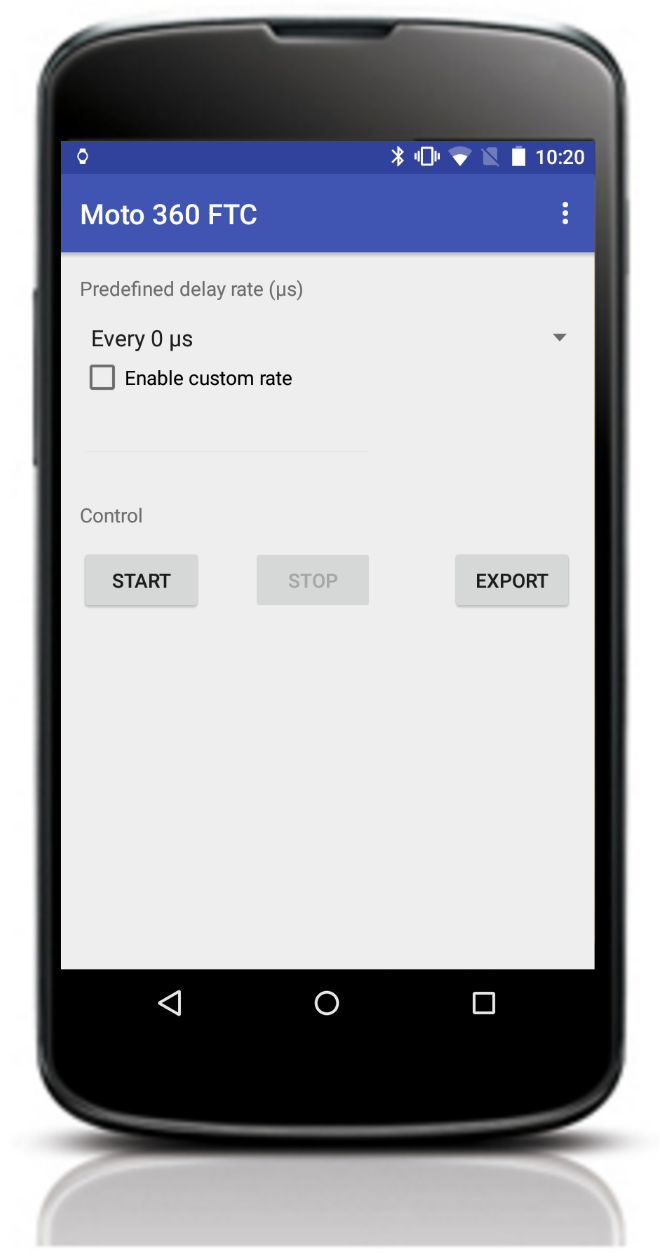
\includegraphics[scale=0.40]{mobile_app} 
        \caption{Mobile App for continuously collecting data from hardware sensors.}
        \label{fig:mobileapp}
    \end{figure}
    
    Initially, we compare the accuracy of heart rate monitoring among the two wearable devices and the fingertip pulse oximeter when the examinee is resting. During the experiment, the wrist and arm should be kept steady. As described in section \ref{sec:Background}, the problem in measuring the heart rate is the motion artifacts. The motion artifacts distort the PPG signal. When the examinee moves, LED and PD of the PPG sensor are moved and the PD doesn’t exactly detect reflected or back scattered light. That’s why PPG signal is distorted. Therefore, we compare the accuracy of heart rate monitoring among the two wearable devices and the fingertip pulse oximeter when the examinee is in regular exercise (i.e. jogging at 5 mile/hr).
    
    As described in section \ref{subsec:HardwareRelatedWork}, to find the relation between the distorted PPG signal and acceleration from each axis of accelerometers, we design the experiments as bellow. First, the examinee wave the arm/wrist left and right along the x-axis respectively, and doesn’t move up and down along the z-axis. The examinee then wave the arm/wrist back and forth along the y-axis. Similarly, the examinee is not allowed to wave the arm up and down along the z-axis. Last, the examinee wave the arm/wrist up and down along the z-axis. To find the relation between the PPG signal and the accelerometer signal during the regular exercise, in the fourth experiment, the examinee is asked to wave the arm/wrist as regular walking.

    
    % Implementation
	% What language, IT infrastructure? What are the pragmatic trade-offs that you had to make? What is the complexity of the implementation – LOC, other metrics? What are the dependencies of your implementation? 

	\subsection{Experiments and Results} %[As much as you need]
	%For each result, explain: what is the goal of the experiment, what you did, then comes the plot, then interpret the plot. Try and have some comparative result, with prior work. 
    
    In this section, we present the experimental results. In all the experiments, the examinee is a healthy male with 6 inch height and 170 pounds weight. 
\\
    
    \textbf{Comparison Analysis}
    
    % Figure 1
    \begin{figure}[h]	
        \centering
        % Comparison Analysis between iWatch, Moto 360, Fingerclip (Resting)
        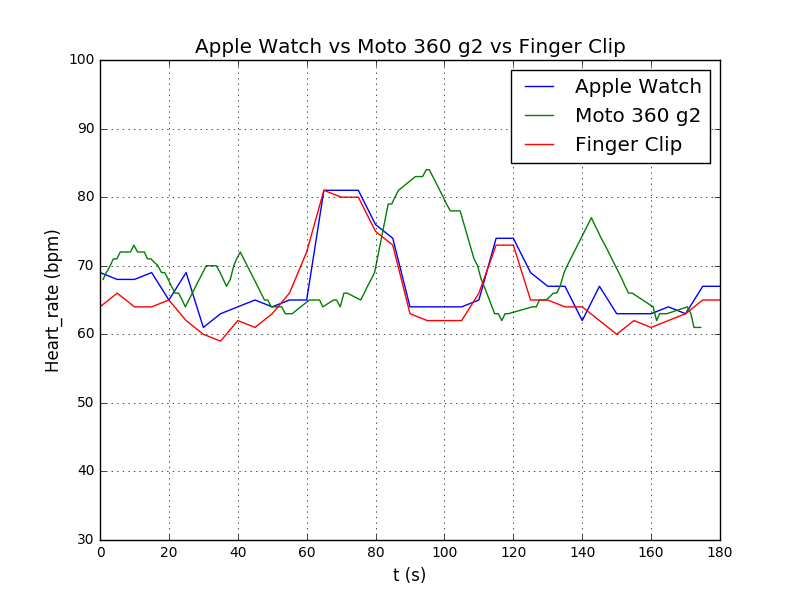
\includegraphics[scale=0.50]{heart_rate_apple_steady} 
        \caption{Resting heart ratio comparison.}
        \label{fig:HeartRateComSteady}
    \end{figure}
    
    % Figure 1
    \begin{figure}[h]	
        \centering
        % Comparison Analysis between iWatch, Moto 360, Fingerclip (motion)
        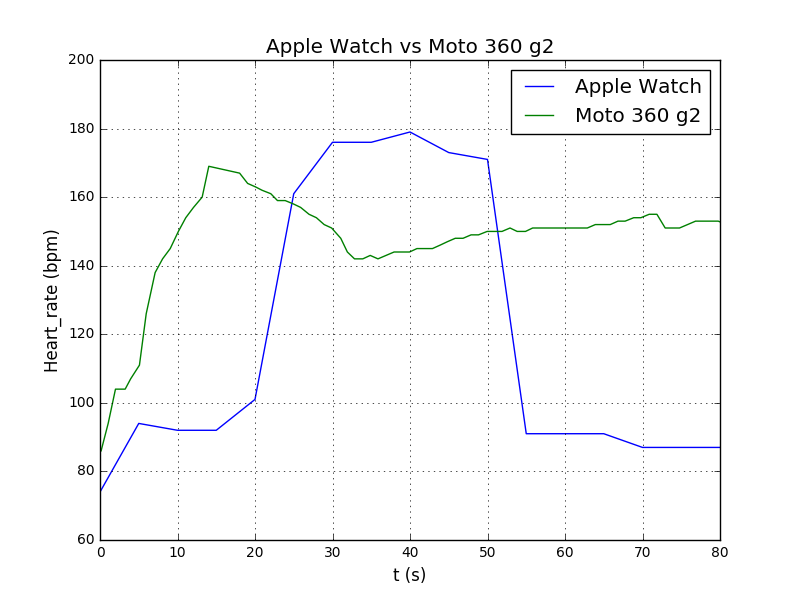
\includegraphics[scale=0.50]{heart_rate_apple_move}
        \caption{Heart rate comparison with Motions. Jogging 5 miles/hour.}
        \label{fig:HeartRateComMove}
    \end{figure}
    
    Fig.~\ref{fig:HeartRateComSteady} shows the comparison experimental results of Moto 360 (2nd Gen.), Apple Watch and the fingertip pulse oximeter when the examinee is resting. The y-axis represents the heart rate (BPM), and the x-axis represents the time (seconds). It is indicated from the plot that both Apple Watch and Motorola Moto 360 (2nd Gen.) present heart rate closed to the reading from fingertip pulse oximeter. However, we find there is a non-negligible delay time for the reading of android wearable. Fig.~\ref{fig:HeartRateComMove} shows the comparison experimental results of the Motorola Moto 360 (2nd Gen.) and Apple Watch when the examinee is jogging at 5 mile/hr. In the case of the fingertip pulse oximeter, the BPM values are not shown since the device does not output lecture on motion. Thus, the values for the heart rate readings before the exercise and after the exercise are 67 BPM and 93 BPM respectively. With this in mind, it is easy to see both Motorola and Apple smartwatches are not accurate due to the motion artifacts. However, the heart rate readings of Apple Watch are more accurate than the readings of Motorola Moto 360 (2nd Gen.).

	\pagebreak
    \textbf{Motion Artifacts Analysis}
    
    Fig.~\ref{fig:X_AccPPG}-~\ref{fig:Z_AccPPG} show the result of experiments of the relation between the PPG signal and moving along each axis. The upper signal is the distorted PPG signal from Motorola wearable. The next waveforms (c), (d) and (e) are the outputs of each x-axis, y-axis and z-axis accelerometers. To show the relation between PPG signal and the acceleration clearly, we used the Pearson correlation coefficient. The correlation coefficient represents interrelation between the signals. The numerical formula of correlation is as follows:    
    
    \begin{equation}
    Cor(x,y)=\frac{1}{m}\frac{\sum\limits_{i=1}^{m}(x_i-\mu_x)(y_i-\mu_y)}{\sigma_x\sigma_y}
    \end{equation}

    
where $\mu$, $\sigma$ are the mean and the standard deviation of the PPG and the acceleration on each axis. The correlation coefficients for each axis are presented in tables 1-3. The experimental results indicate that the PPG signal is much correlated with x-axis acceleration when disrupted PPG signal is delayed by 0.2s. That means the motion reflects a little delayed time and the noise which corrupts generate from x-axis acceleration. In fig.~\ref{fig:XYZ_AccPPG} and table~\ref{table:XYZ_AccPPG}, we show the results for the relation between the PPG signal and the accelerometer data on each axis when the examinee is in regular walking. Apparently, the results are consistent with what we describe earlier.
    
    Next, we test how much x-axis acceleration has an effect on the heart rate monitoring. In Fig. 8, we show the heart rate (rpm) on the y-axis and the time (s) on the x-axis. We show three different scenarios when x-axis acceleration are \SI[per-mode=symbol]{2}{\metre\per\second\squared}, \SI[per-mode=symbol]{4}{\metre\per\second\squared} and \SI[per-mode=symbol]{8}{\metre\per\second\squared}. The experimental results indicate that the lower the x-axis acceleration, the higher the accuracy of heart rate monitoring.
    
    % Figure 1
    \begin{figure}[ht]	
        \centering
        % PPG Signal with acc on X-axis
        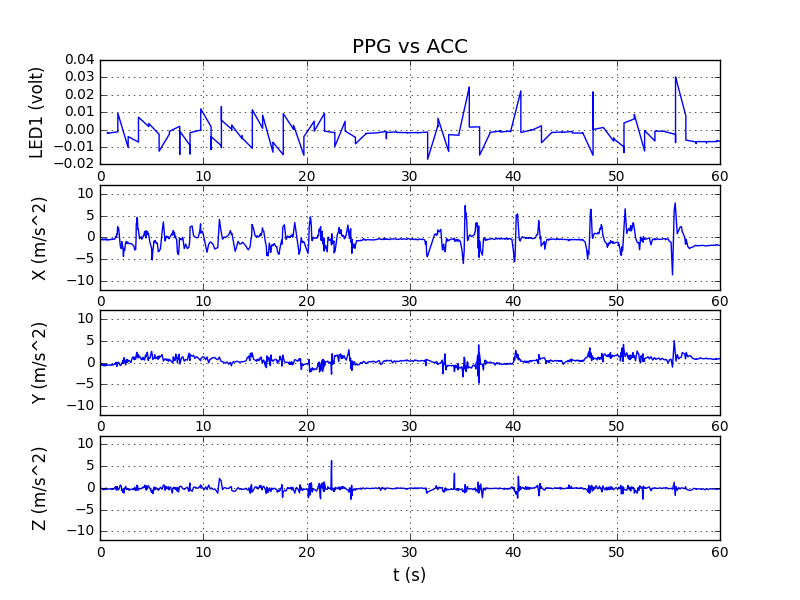
\includegraphics[scale=0.50]{x_acc_ppg_acc_19} 
        \caption{Plot of PPG signal with acceleration on X-axis.}
        \label{fig:X_AccPPG}
    \end{figure}
    
    \begin{table}[ht]
	\centering
        \caption{}
		\label{table:X_AccPPG}
		\begin{tabular}{ l l|r|r|r|r| }
			\cline{3-6}
            & & \multicolumn{4}{|c|}{Delay Time of PPG signal} \\
            \cline{3-6}
            	& & 0s & 0.1s & 0.2s & 0.3s  \\
			\hline
            \multicolumn{1}{|c|}{\multirow{3}{*}{Acceleration}} 
            	& X axis & 0.36  & 0.47 & \textbf{0.53} & 0.44  \\
            \cline{2-6}
            \multicolumn{1}{|c|}{} 
            	& Y axis & -0.02 & 0.01 & 0.04 & 0.02  \\
            \cline{2-6}
            \multicolumn{1}{|c|}{} 
            	& Z axis & 0.02  & 0.01 & 0.08 & 0.06  \\
			\hline
		\end{tabular}
	\end{table}

    % Figure 1
    \begin{figure}[h]	
        \centering
        % PPG Signal with acc on Y-axis
        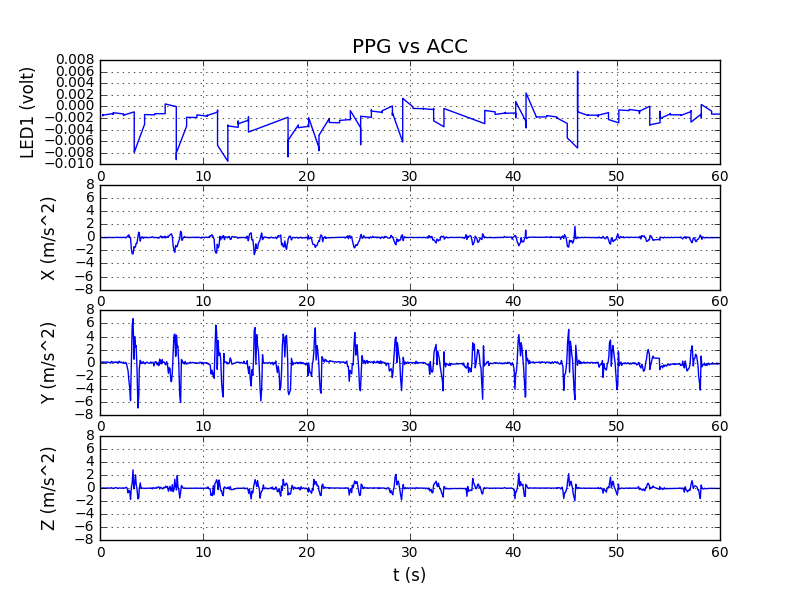
\includegraphics[scale=0.50]{y_acc_ppg_acc_17} 
        \caption{Plot of PPG signal with acceleration on Y-axis.}
        \label{fig:Y_AccPPG}
    \end{figure}
    
    \begin{table}[ht]
	\centering
        \caption{}
		\label{table:Y_AccPPG}
		\begin{tabular}{ l l|r|r|r|r| }
			\cline{3-6}
            & & \multicolumn{4}{|c|}{Delay Time of PPG signal} \\
            \cline{3-6}
            	& & 0s & 0.1s & 0.2s & 0.3s  \\
			\hline
            \multicolumn{1}{|c|}{\multirow{3}{*}{Acceleration}} 
            	& X axis & 0.09  & 0.47  & 0.32  & \textbf{0.42}  \\
            \cline{2-6}
            \multicolumn{1}{|c|}{} 
            	& Y axis & 0.08  & 0.01  & -0.11 & -0.20  \\
            \cline{2-6}
            \multicolumn{1}{|c|}{} 
            	& Z axis & 0.07  & -0.02 & -0.14 & -0.23  \\
			\hline
		\end{tabular}
	\end{table}
    
    % Figure 1
    \begin{figure}[h]	
        \centering
        % PPG Signal with acc on Z-axis
        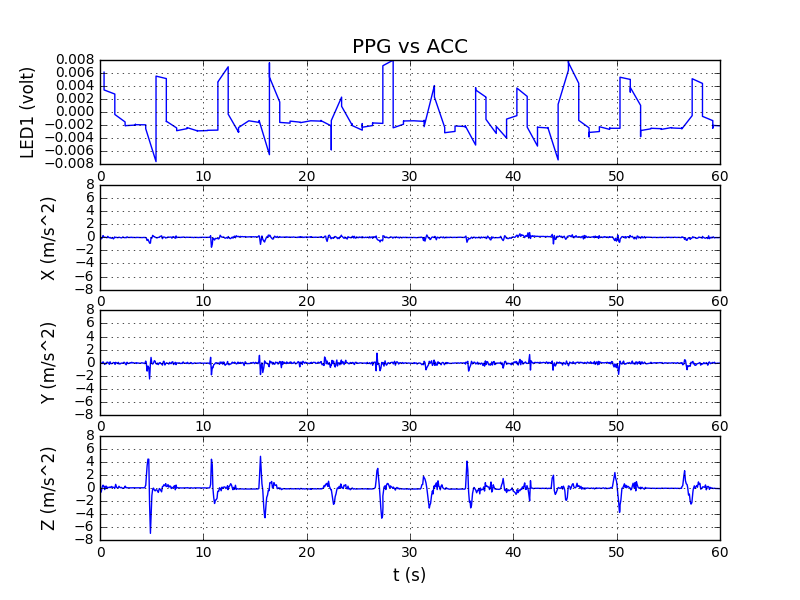
\includegraphics[scale=0.50]{z_acc_ppg_acc_12} 
        \caption{Plot of PPG signal with acceleration on Z-axis.}
        \label{fig:Z_AccPPG}
    \end{figure}
    
    \begin{table}[ht]
	\centering
        \caption{}
		\label{table:Z_AccPPG}
		\begin{tabular}{ l l|r|r|r|r| }
			\cline{3-6}
            & & \multicolumn{4}{|c|}{Delay Time of PPG signal} \\
            \cline{3-6}
            	& & 0s & 0.1s & 0.2s & 0.3s  \\
			\hline
            \multicolumn{1}{|c|}{\multirow{3}{*}{Acceleration}} 
            	& X axis & 0.08  & 0.08  & 0.08  &  0.08  \\
            \cline{2-6}
            \multicolumn{1}{|c|}{} 
            	& Y axis & 0.02  & 0.01  & 0.02 & -0.01  \\
            \cline{2-6}
            \multicolumn{1}{|c|}{} 
            	& Z axis & 0.06  & 0.003 & -0.07 & -0.15  \\
			\hline
		\end{tabular}
	\end{table}
    
    % Figure 1
    \begin{figure}[h]	
        \centering
        % PPG Signal with acc on XYZ-axis
        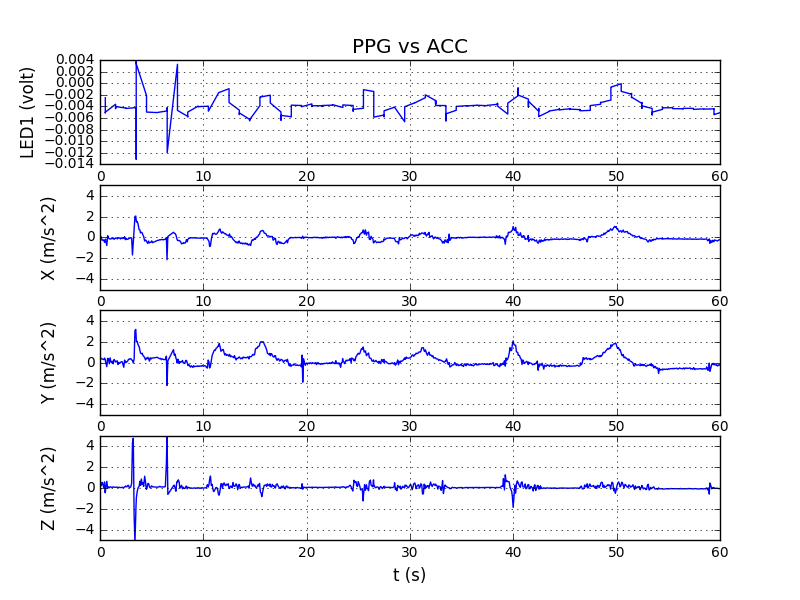
\includegraphics[scale=0.50]{xyz_acc_ppg_acc_8} 
        \caption{Plot of PPG signal with acceleration on all axis (X, Y, Z).}
        \label{fig:XYZ_AccPPG}
    \end{figure}
    
    \begin{table}[ht]
	\centering
        \caption{}
		\label{table:XYZ_AccPPG}
		\begin{tabular}{ l l|r|r|r|r| }
			\cline{3-6}
            & & \multicolumn{4}{|c|}{Delay Time of PPG signal} \\
            \cline{3-6}
            	& & 0s & 0.1s & 0.2s & 0.3s  \\
			\hline
            \multicolumn{1}{|c|}{\multirow{3}{*}{Acceleration}} 
            	& X axis & 0.63  & 0.72  & \textbf{0.78}  &  0.77  \\
            \cline{2-6}
            \multicolumn{1}{|c|}{} 
            	& Y axis & 0.48  & 0.55  & 0.59 &  0.57  \\
            \cline{2-6}
            \multicolumn{1}{|c|}{} 
            	& Z axis & 0.03  & -0.05 & -0.13 & -0.12  \\
			\hline
		\end{tabular}
	\end{table}
    
    % Figure 1
    \begin{figure}[h]	
        \centering
        % Comparison Analysis between iWatch, Moto 360, Fingerclip
        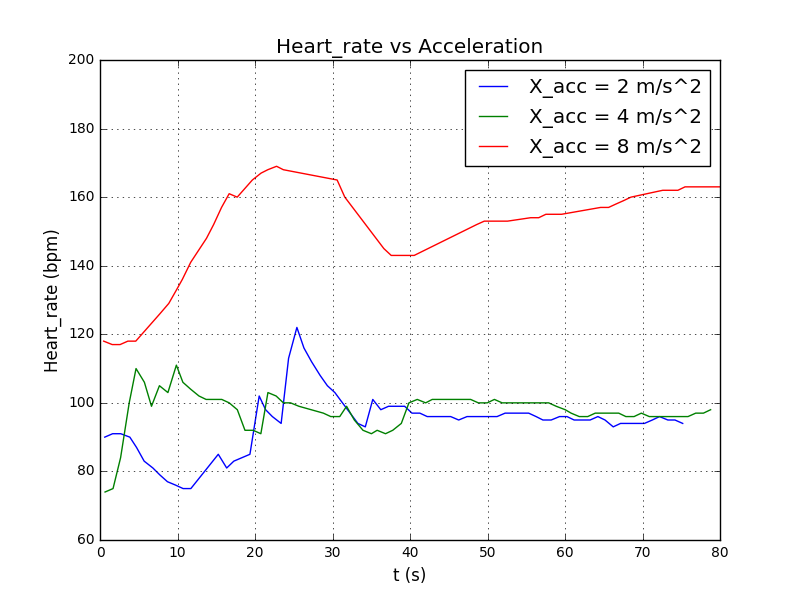
\includegraphics[scale=0.50]{heart_rate_com} 
        \caption{Plot of PPG signal with Acceleration on X-Axis.}
        \label{fig:HeartRateCom}
    \end{figure}
    
    \section{Software} \label{sec:Software}
    
    \subsection{Related Work} \label{subsec:SoftwareRelatedWork}
    % Existing solutions
    
    Android Wear 1.0, which comes with the Motorola Moto 360 (2nd Gen.), was released on 2014. The next version of the OS, Android Wear 2.0, was pushed back from last October to next year. Even thought, Android has the largest share in the smart phone market, with 87\%~\cite{IDC2016PhoneMarket}, that dominance has not translated to the wearable area. Still, Android Wear is considered a popular OS on wearable devices. However, as we showed on the previous section, Motorola Moto 360 (2nd Gen.) is not as accurate as Apple Watch.
    
   To verify the overall reliability of the Android wearable devices we devise that a fuzz testing technique will be helpful. Fuzz testing involves to randomly generating or mutating well-formed input data and test the application using this input. Fuzzing is able to identify most common errors and potential vulnerabilities quickly and cost effectively. Thus, by applying fuzzing we will be able to verify how reliable is the software on Motorola Moto 360 (2nd. Gen.)
   
   Initially, our solution was based on fuzz test the input data of sensors, and inject that input on the Google Fit API, to test the reliability of Fitness and Health apps. Basically, the idea is to stress the apps using a black box approach. The test could conducted either using an existing tool, or implementing a tool. At first instance, the approach was to build a partial fuzz tester, just focused on the generation of the input data, and then inject that input on the target.
   
   For implementing the tool, two different approach were evaluated:
   
   \begin{itemize}
   \item \textbf{Use data injection mode}. Android has a data injection mode available on \texttt{SensorManager} class. Using the mode, the data collected by hardware sensors is ignored; instead, the data injected is considered by the \texttt{Sensor}. This mode should be activate through the Android Debug Bridge (ADB) tool, as shown on listing~\ref{lst:injection}. Unfortunately, this mode is not only available by third parties, but the OS.  Which means that we would need to modify the Android Wear OS to take advantage of this mode. For this reason, this option was discarded.
   
   \begin{lstlisting}[captionpos=b, caption={Enabling injection mode.}, label={lst:injection}, language=Java]
adb shell dumpsys sensorservice data_injection android.sensor.accelerometer
	\end{lstlisting}
    
   \item \textbf{Exploit the fact Android is based on Linux.} In Unix-like operating systems, special files that acts as interface for device driver are located on \texttt{/dev/input}. All device's input, including sensors, can be found on that directory; which means that we can interact with them using \texttt{sendevent} and \texttt{getevent} ADB's commands. This is exploited by  ~\cite{mohamed2016smashed} to read and write to different sensors. However, the test that we conducted revealed that this vulnerability or behavior is not longer present on the Android OS (neither Android Wear OS) starting the Lollipop version (5.0). Then, this approach was also discarded.
	\end{itemize}  

	Due the impossibility to find a viable way to fuzz the sensor data, we decide to use an existing tool. There are many fuzzers on Linux, but a handful tools on Android. Although there are no specialized tool for Android Wear, since the OS is based on Android, the same tools can be used on both OS. The most popular tools are Android official tools, Monker UI and Monkey Runner, which offers limited features. More advanced tools include: ~\cite{Cui2015}, ~\cite{Machiry2013}, ~\cite{Ye2013}. However, none of the tools reviewed offers the possibility to fuzz sensor data. Thus, we decided to change our initial scope to test the reliability of Android Wear software. Instead of fuzz the sensor data, we decided to apply a fuzz test to all the Android Wear built-in apps using one of the official Android test tools, Monkey UI. 
   
   
    \subsection{Design and Implementation} \label{subsec:SoftwareDesignImple} %[1-3 pages]
	% Design
    % 3.1 High-level conceptual figure of how your solution works
	% 3.2 Workflow of how your solution works – the detailed pieces will come in the next section – you can
	% 3.3 What kinds of failures or attacks is your solution meant to handle
	% 3.4 One or two common use cases – how an end user will use your solution 
    Motorola Moto 360 (2nd Gen.) includes 45 packages, which only 14 are susceptible to be tested. Android Monkey UI can only be used to stress-test the UI (user interface) of applications. Thus, apps must have a Main Activity defined, which means that others app such as services cannot be tested. The testing tool generates pseudo random streams of user events (e.g. click, touches or gestures)~\cite{AndroidUITester}. The packages that were tested are listed on table~\ref{table:FuzzPackage}.
    
    \begin{table}[ht]
	\centering
        \caption{}
		\label{table:FuzzPackage}
		\begin{tabular}{ |l|l| }
			\hline
				App Name         & package \\
			\hline
				Moto Body        & com.motorola.omni \\
				Flashlight       & com.google.android.clockwork.flashlight \\
				Settings         & com.google.android.apps.wearable.settings \\
				Clock            & com.google.android.deskclock \\
				Music            & com.google.android.music \\
				Maps             & com.google.android.apps.maps \\
				Fitness          & com.google.android.apps.fitness \\
				Google Services  & com.google.android.gms \\
				Reminders        & com.google.android.wearable.reminders \\
				Photos           & com.google.android.apps.wearable.phone \\
				Translate        & com.google.android.apps.translate \\
				Wearable App     & com.google.android.wearable.app \\
				Keep             & com.google.android.keep \\
				Talk             & com.google.android.talk \\
			\hline
		\end{tabular}
	\end{table}	

	The stress test consisted on running 4000 trials for each package. For the test, the developer mode on the the Motorola Moto 360 (2nd Gen.) was enabled. Besides, the debugging via bluetooth was activated. For the experiments we used the default sample distribution of Android Monkey UI, as shown in fig.~\ref{fig:FuzzEvents}. If an application crashed, the test will be repeated until complete the required 4000 trials for the package. The test were launched manually, using an script.
    
    % Figure 1
    \begin{figure}[h]	
        \centering
        % Distribution of Fuzz Events
        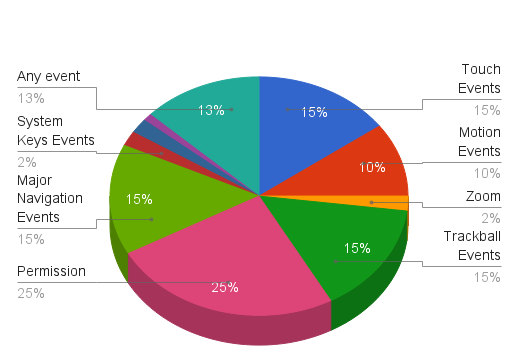
\includegraphics[scale=0.60]{fuzz_events} 
        \caption{Distribution of Sample Events.}
        \label{fig:FuzzEvents}
    \end{figure}
	
    % Implementation
	% What language, IT infrastructure? What are the pragmatic trade-offs that you had to make? What is the complexity of the implementation – LOC, other metrics? What are the dependencies of your implementation? 

	\subsection{Experiments and Results} %[As much as you need]
	%For each result, explain: what is the goal of the experiment, what you did, then comes the plot, then interpret the plot. Try and have some comparative result, with prior work. 
    
    During the experiments, we observed that the only apps that crashed were the fitness apps: Moto Body and Google Fitness. Then, we decided to extend the test and continue stressing those apps by running 10000 on each apps. As we an observe on figure~\ref{fig:FuzzTrials}, at the end of the experiment, Moto Body crashed 6 times, while the Google Fitness crashed 1 time.
    
	% Figure 1
    \begin{figure}[h]	
        \centering
        % Fuzz test results on fitness apps
        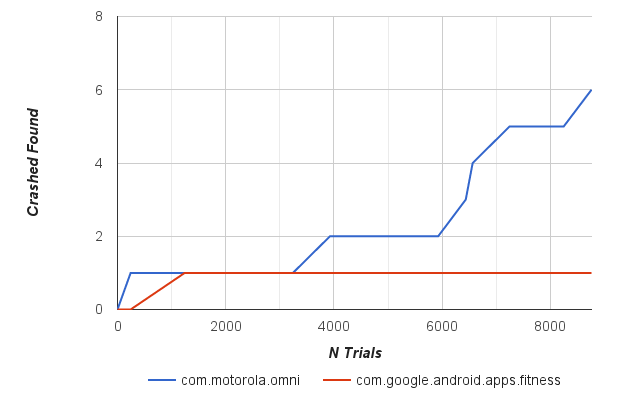
\includegraphics[scale=0.50]{fuzz_crashs} 
        \caption{Crashes per trials on fitness apps.}
        \label{fig:FuzzTrials}
    \end{figure}
    
    Finally, we can conclude that fitness apps are less reliable than the rest of the apps on the Android Wear. Specifically, the Moto Body app release by Motorola is vulnerable than the Google Fitness app. All the errors reported on the Moto Body app were NullPointerException, either for attempting to read a field with null value or invoke a method using a null object reference.
    
	%\section{Discussion}
	% Here talk of things that your solution does not address straight away, but can be tweaked to handle. Point out weaknesses of your solution and how you would address them
		
	\section{Conclusion} \label{sec:Conclusion}
	% Summarize the main contributions of the work and what further work someone should do to make the solution better. 
	% The conclusion goes here.
    In this project, we analyzed the reliability of wearable device from the hardware and software perspective. For hardware perspective, we compare the reliability between the Motorola Moto 360 (2nd. Gen), Apple iWatch and the Santamedical Generation 2 SM-165 Fingertip Pulse Oximeter. We showed that the accuracy between the Apple iWatch and the SM-165 Fingertip is very close. In contrast, in the Motorola Moto 360 (2nd Gen.) there is a delay time. Also, the experiments showed that there accuracy of all three device is very accurate during resting, and less accurate with motion body. The more significant of the motion body, the less of the accuracy.
    
    Furthermore, the PPG signal is affected body motion, and particularly from the acceleration on the X axis. Thus, the PPG signal is more correlated to the X axis acceleration than any of the other axis. The motion reflects a little delayed time (about 0.2s) on PPG signal. 
    
    Finally, for the software perspective, we realized fuzz testing to Motorola Moto 360 (2nd Gen.) built-in apps. From the test, we can conclude that the fitness apps are less reliable than the rest, specially the Moto Body app.
    
    \section{Future Work} \label{sec:FutureWork}
    % Future work goes here.
    In the experiment section, we showed that the heart rate monitor from the Motorola Moto 360 (2nd Gen.) is less accurate on the presence of body motion. In this sense, the accuracy can be improved by implementing an algorithm to discard untrustable data, and cancel the noise using machine learning techniques. Besides, further experiments can be done in the following areas:
    \begin{itemize}
    \item \textit{Rhythmic Movements}. Compare the impacts of rhythmic movements, such as running, cycling, playing tennis (or any other sport), on the heart rate monitor.
    \item \textit{Fuss Tester}. Build a fuzz testing tool capable of fuzz sensor data (either generate the data randomly or mutate from specific patterns), and use it to check the reliability of the Google Fit API. Also, apply test using white box testing instead of a black box, as was done for this project.
    \end{itemize}
    
	% conference papers do not normally have an appendix
	
	
	% use section* for acknowledgment
	%\section*{Acknowledgment}
	
	
	%The authors would like to thank...
	
	
	
	
	
	% trigger a \newpage just before the given reference
	% number - used to balance the columns on the last page
	% adjust value as needed - may need to be readjusted if
	% the document is modified later
	%\IEEEtriggeratref{8}
	% The "triggered" command can be changed if desired:
	%\IEEEtriggercmd{\enlargethispage{-5in}}
	
	% references section
	
	% can use a bibliography generated by BibTeX as a .bbl file
	% BibTeX documentation can be easily obtained at:
	% http://mirror.ctan.org/biblio/bibtex/contrib/doc/
	% The IEEEtran BibTeX style support page is at:
	% http://www.michaelshell.org/tex/ieeetran/bibtex/
	% \nocite{*}
	\bibliographystyle{IEEEtran}
	% argument is your BibTeX string definitions and bibliography database(s)
	\bibliography{IEEEabrv,ref}
	%
	% <OR> manually copy in the resultant .bbl file
	% set second argument of \begin to the number of references
	% (used to reserve space for the reference number labels box)
	% \begin{thebibliography}{1}
	% 	
	%	\bibitem{IEEEhowto:kopka}
	%	H.~Kopka and P.~W. Daly, \emph{A Guide to \LaTeX}, 3rd~ed.\hskip 1em plus
	%	0.5em minus 0.4em\relax Harlow, England: Addison-Wesley, 1999.
	%	
	% \end{thebibliography}
	
	
	
	
	% that's all folks
\end{document}